%SUPERFICIES FORESTALES

%----------------------------------------------------------
\section{Entorno de trabajo}

    El entorno de trabajo es el medio por el cual el usuario interactúa con el sistema para poder gestionar la información referente a las Escuelas inscritas en el Programa de Acreditación de Escuelas Ambientalmente Responsables. En este capítulo se describe el comportamiento y los elementos que conforman el entorno de 
    trabajo del PAEAR, como son: la disposición de los elementos principales y comunes de las pantallas, los colores, la iconografía, componentes, etc. \bigskip

    \begin{objetivos}
      \item Describir las áreas principales del entorno de trabajo.
      \item Describir la iconografía utilizada en las pantallas.
      \item Describir el mapa de navegación del sistema.
      \item Describir los componentes principales de las pantallas, tales como: controles de entrada, datos obligatorios, separadores, tablas de resultados, entre otros.
    \end{objetivos}
\\\\\\\\\\\\\\\\
%----------------------------------------------------------

\subsection{Diseño}

  El diseño de las pantallas del sistema sigue un enfoque minimalista que permite a los usuarios trabajar sin gran dificultad y sin distracción. 
  Las pantallas son consistentes, ya que tienen un diseño homogéneo y cuentan con componentes comunes; la consistencia facilita al usuario la interacción
  con el sistema a medida que hace uso del mismo. En la figura~\ref{fig:entornoDeTrabajo} se muestran los elementos principales que conforman las pantallas del sistema, 
  dichos elementos se describen a continuación:

  \begin{figure}[ht!]
      \begin{center}
	  \fbox{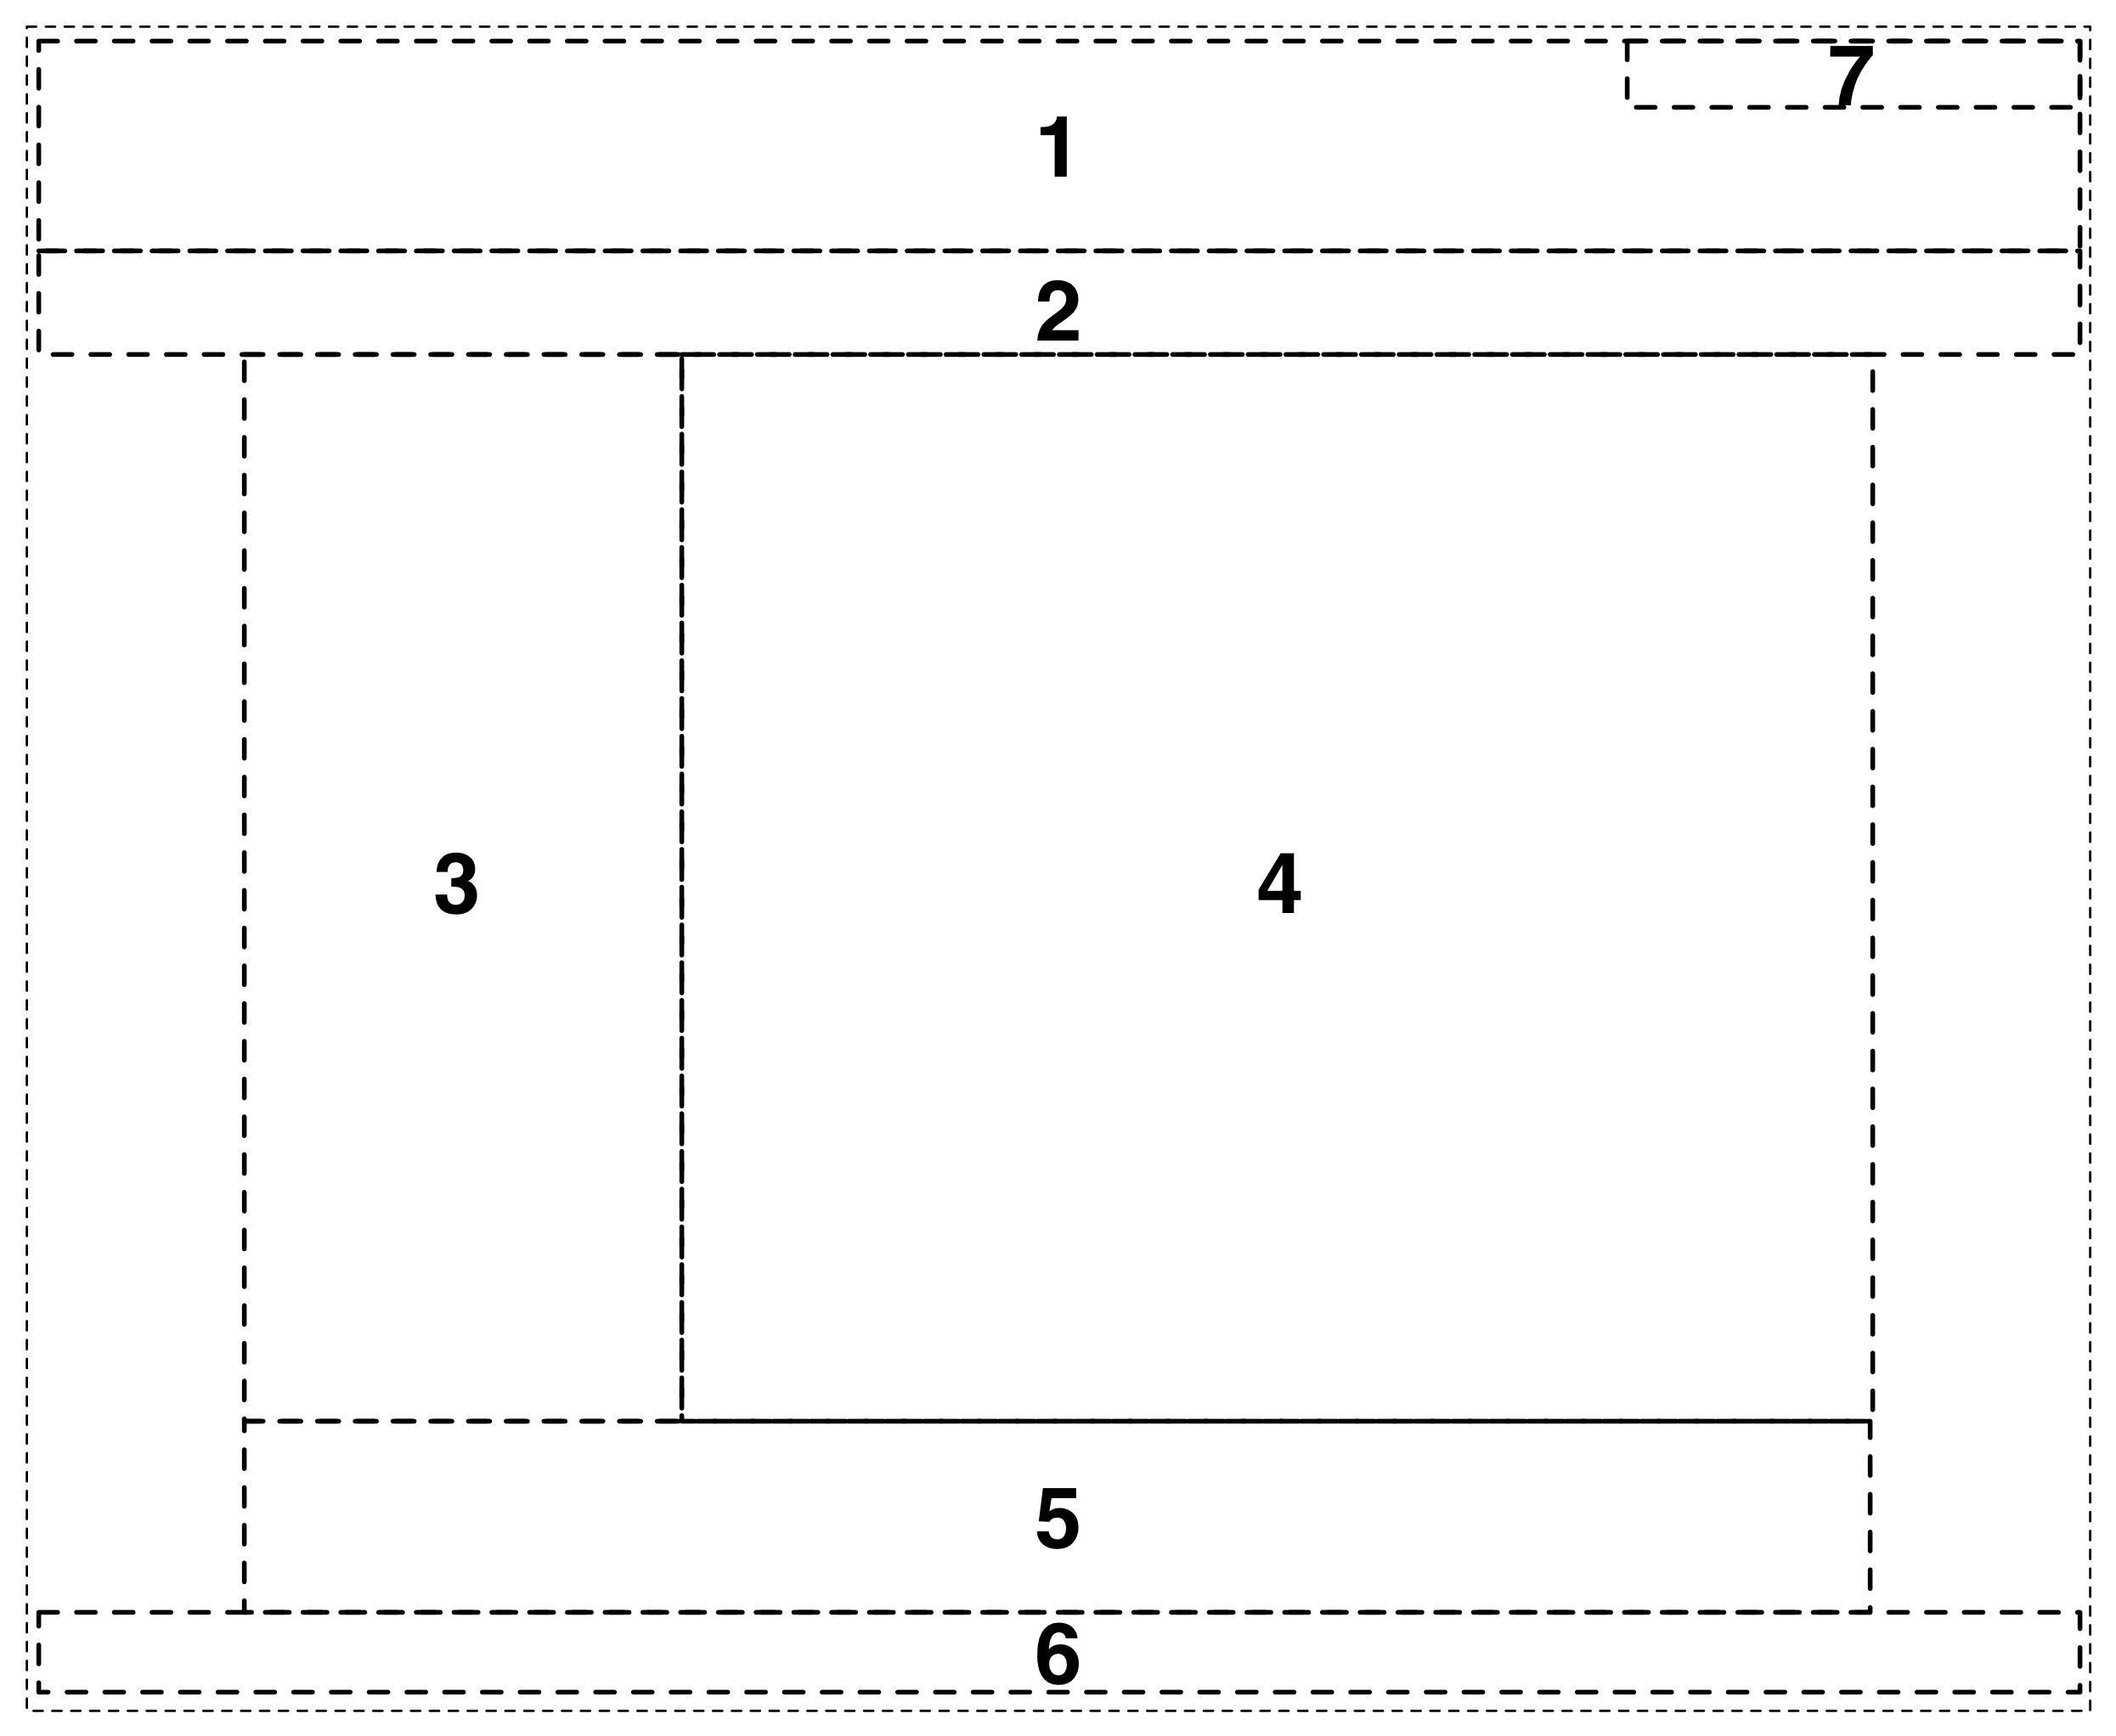
\includegraphics[width=.8\textwidth]{images/pantallas/general/layout}}
	  \caption{Entorno de trabajo del sistema.}
	  \label{fig:entornoDeTrabajo}
      \end{center}
  \end{figure}

    \begin{enumerate}
        \item {\bf Encabezado:} el encabezado tiene la finalidad de mostrar la imagen institucional de la dependencia a la cual pertenece, es decir, la imagen institucional del Gobierno del Estado de México.
        \begin{itemize}
            \item Ancho: $100\%$ del ancho de la ventana del navegador.
            \item Alto: $90px$.
        \end{itemize}

        \item {\bf Menú horizontal:} muestra las opciones generales de navegación para los distintos tipos de usuarios.
        \begin{itemize}
            \item Ancho: $100\%$ del ancho de la pantalla del navegador.
            \item Alto: $40px$.
        \end{itemize}
        
        \item {\bf Menu vertical:} es el área destinada al menú vertical que contendrá los vínculos necesarios para ingresar a las opciones que proporcione el sistema a cada uno de los distintos perfiles de usuarios.
        
        El menú vertical no se encontrará visible para los perfiles de usuario que no requieran del mismo y este espacio será utilizado por el área de trabajo (ver siguiente punto).
        
        \begin{itemize}
            \item Ancho: $20\%$ del ancho de la pantalla del navegador.
            \item Alto: autoajustable al contenido.
        \end{itemize}
        
        \item {\bf Área de trabajo:} en esta sección los usuarios visualizarán los elementos que el sistema proporciona para la realización de las tareas contempladas en el mismo. Aquí se desplegarán formularios para captura, tablas, imágenes, gráficas y demás elementos contenidos en el sistema.\\
        
        El contenido en esta sección se visualizará centrada con base en el ancho y alineado a la parte superior de la misma. Todas las pantallas deberán contar con un título alineado al centro del área de trabajo. 
        \begin{itemize}
            \item Ancho: ancho mínimo $500px$, $65\%$ del ancho de la ventana del navegador web cuando el menu vertical esta visible o el $80\%$ del ancho de la ventana del navegador web en ausencia del menu vertical.
            \item Alto: autoajustable al contenido con un mínimo de $400px$.
        \end{itemize}
        
        \item {\bf Pie:} esta sección contendrá la información de contacto de la unidad correspondiente de la Secretaría del Medio Ambiente del Gobierno del Estado de México.
        \begin{itemize}
            \item Ancho: $80\%$ del ancho de la ventana del navegador.
            \item Alto: $84px$
        \end{itemize}
        
        \item {\bf Información legal:} muestra una leyenda con información legal referente a la propiedad y uso del sistema.
        \begin{itemize}
            \item Ancho: $100\%$ del ancho de la ventana del navegador.
            \item Alto: 24px.
        \end{itemize}
        
        \item {\bf Información de sesión:} esta sección será visible sólo cuando un usuario ingrese al sistema. En ella se mostrarán las opciones para cambiar la contraseña de acceso al mismo, el nombre de usuario y el cierre de sesión.
        \begin{itemize}
            \item Ancho: ajustable al contenido.
            \item Alto: $30px$;
        \end{itemize}
    \end{enumerate}

  
%  	\begin{enumerate}
%		\item {\bf Datos de Sesión:} Esta sección será visible solo cuando un actor ingrese al sistema. En ella se mostrarán los datos del actor que haya iniciado sesión, así como las opciones para el cierre de sesión y el 
%		cambio de contraseña.
		
%		\item {\bf Baner de la página:} Tiene la finalidad de mostrar la imagen institucional de la dependencia a la cual pertenece el sistema. Aquí se muestran los logotipos de la Secretaría del Medio Ambiente y del 
%		Gobierno del Estado de México.
		
%		\item {\bf Menú superior:} Muestra las opciones generales de navegación para los diferentes tipos de actores.
		
%		\item {\bf Área de trabajo:} En esta sección los actores visualizarán los elementos que el sistema proporciona para la realización de las tareas contempladas en el mismo. Aquí se desplegarán formularios para 
%		captura, tablas, imágenes, gráficas y demás elementos contenidos en el sistema. La documentación de las pantallas se explica a partir de esta sección.
		
%		\item {\bf Pie de página:} En esta sección aparecen los datos de contacto de la  Unidad de Información, Planeación, Programación y Evaluación de la Secretaría del Medio Ambiente del Gobierno del Estado de México y 
%		los del soporte técnico del sistema.
		
%		\item {\bf Información legal:} Muestra una leyenda con información legal referente a la propiedad y uso del sistema.
			
%	\end{enumerate}


%----------------------------------------------------------
\subsection{Pantalla de bienvenida}
\label{ch:Interaccion:PantallaBienvenida}

En la figura \ref{fig:inicio} se muestra la pantalla de bienvenida, en la cual se mostrará el nombre completo del usuario, así como una leyenda de bienvenida.
\begin{figure}[htbp!]
    \begin{center}
	\fbox{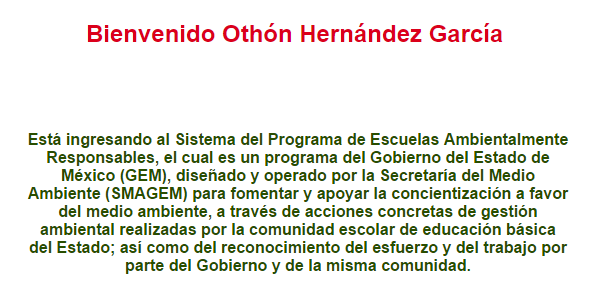
\includegraphics[width=.8\textwidth]{images/inicio.png}}
	\caption{Pantalla de bienvenida.}
	\label{fig:inicio}
	\cdtLabel{fig:inicio}{}
    \end{center}
\end{figure}

%----------------------------------------------------------

\subsection{Componentes utilizados}

  \subsubsection{Pantalla emergente}
    Algunos mensajes se muestran en pantallas emergentes, las cuales cuentan con dos botones: \cdtButton{Aceptar} y \cdtButton{Cancelar}, que permiten confirmar la acción que se muestra en el mensaje.
    En la figura \ref{fig:pantallaEmergente} se muestra una pantalla emergente de ejemplo.
      \begin{figure}[htbp!]
        \centering
	  \fbox{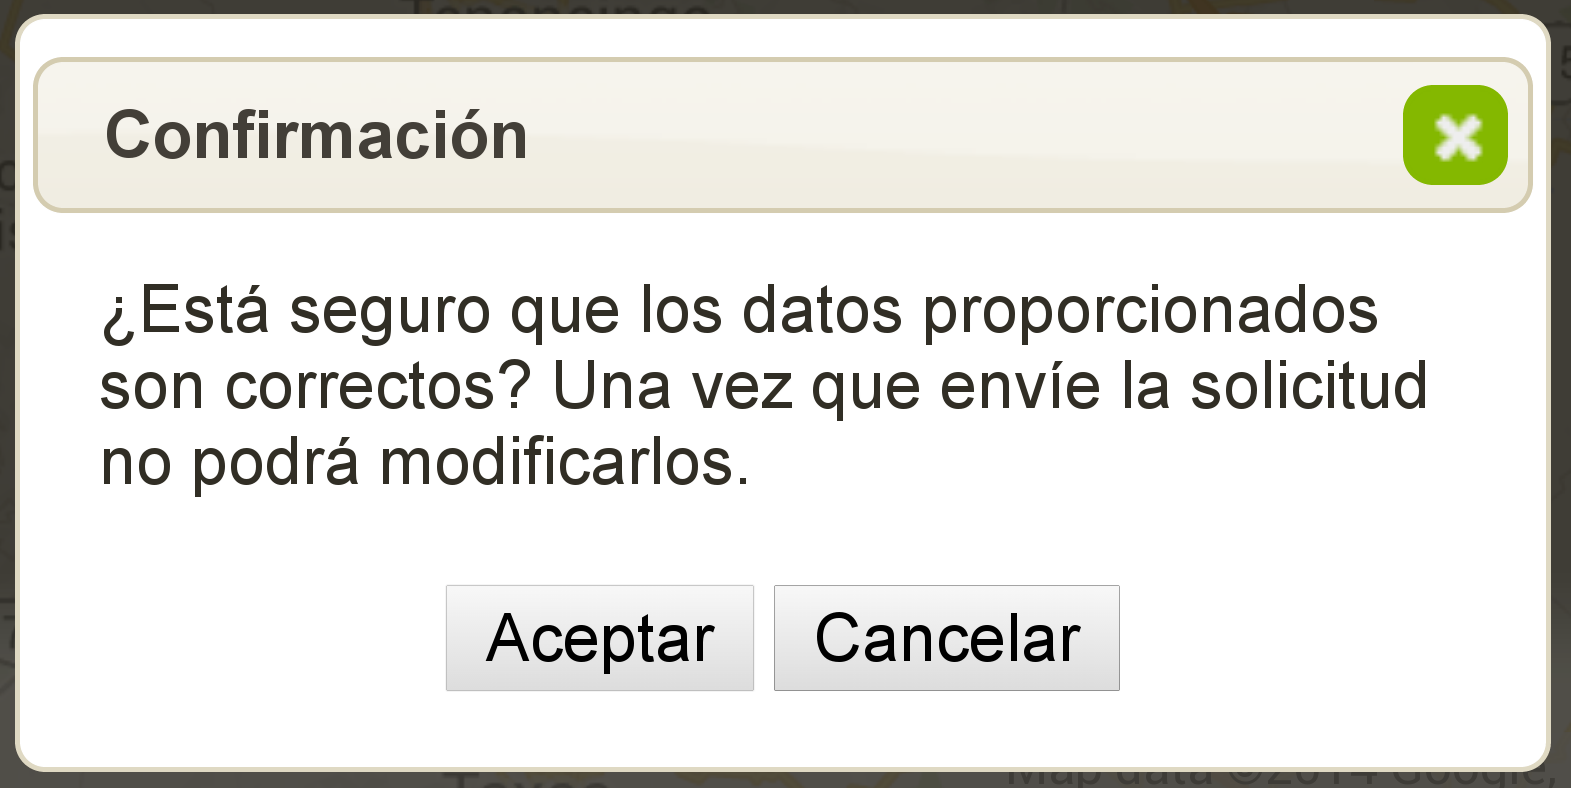
\includegraphics[width=.7\textwidth]{images/pantallas/general/pantallaEmergente.png}}
	  \caption{Pantalla emergente}
	  \label{fig:pantallaEmergente}
	  \cdtLabel{fig:pantallaEmergente}{}
      \end{figure}
  
%----------------------------------------------------------
\subsection{Datos de sesión}
\label{ch:Interaccion:DatosSesion}

En la figura \ref{fig:sesion} se muestra la sección ``Datos de Sesión'', en la cual se mostrará el nombre completo del usuario, así como las opciones para cerrar sesión y cambiar contraseña.
\begin{figure}[htbp!]
    \begin{center}
	\fbox{
\includegraphics[width=\textwidth]{images/datosSesion.png}}
	\caption{Datos de sesión}
	\label{fig:sesion}
	\cdtLabel{fig:sesion}{}
    \end{center}
\end{figure}


\subsection{Iconografía}

  En las pantallas se utilizan diversos íconos para denotar las operaciones que el actor puede realizar sobre el sistema. Los íconos se diseñaron con base en los perfiles de actor y en la operación que podrán realizar 
  después del evento {\it clic} sobre ellos.  A continuación se describe la la funcionalidad de cada uno de ellos:\\\\

  \begin{UClist}
    \UCli \botKo: Permite eliminar un registro del sistema, por ejemplo: un integrante de línea de acción, una actividad en el plan de acción, etc. Al utilizar este ícono no se podrá recuperar la información eliminada. 
%    \UCli \botOk: Se utiliza para aprobar la solicitud de inscripción de una escuela al programa.
%     \UCli \botReg Se utiliza para solicitar el registro de información en el sistema, por ejemplo: un nuevo integrante de línea de acción, información correspondiente al diagnoóstico, etc. 
    \UCli \botEdit: Permite modificar un registro del sistema, por ejemplo: información de un integrante de línea de 		acción, información de la comunidad escolar, etc. Al utilizar este ícono no se podrá recuperar la información  			modificada.
    \UCli \botBus: Se utiliza para buscar información en el sistema, por ejemplo: la información de una escuela por medio de su clave de centro de trabajo.
    \UCli \botAddClip: Se utiliza para adjuntar archivos solicitados por el sistema, por ejemplo: el nombramiento del director de una escuela que se registra para formar parte del programa.
    \UCli \botV: Se utiliza para visualizar información existente en el sistema, por ejemplo: los datos del coordinador del programa.
    \UCli \botDescargar: Se utiliza para descargar un documento del sistema, por ejemplo: la carta compromiso de cierta escuela registrada.
    \UCli \botCalendar: Se utiliza para ingresar una fecha por medio de un calendario.
    \UCli \botReg: Permite administrar inventarios de fauna y de flora.
    \UCli \botMetas: Permite registrar el avance de una meta asociada a una línea de acción.
    \UCli \botAvanceObj: Permite el acceso a la administración de metas de un objetivo en el seguimiento del plan de ación.
    \UCli \botVer: Permite el acceso a la administración de metas y acciones respectivamente.
    \UCli \botAutoAjus: Permite registrar el avance de acciones asociadas a una meta.
    
  \end{UClist}


%----------------------------------------------------------
\subsection{Componentes utilizados}

  \subsubsection{Pantalla emergente}
    Algunos mensajes se muestran en pantallas emergentes, las cuales cuentan con dos botones: \cdtButton{Aceptar} y \cdtButton{Cancelar}, que permiten confirmar o  rechazar la acción que se muestra en el mensaje así como se muestra en la figura \ref{fig:pantallaEmergente}.
      \begin{figure}[htbp!]
	\begin{center}
	  \fbox{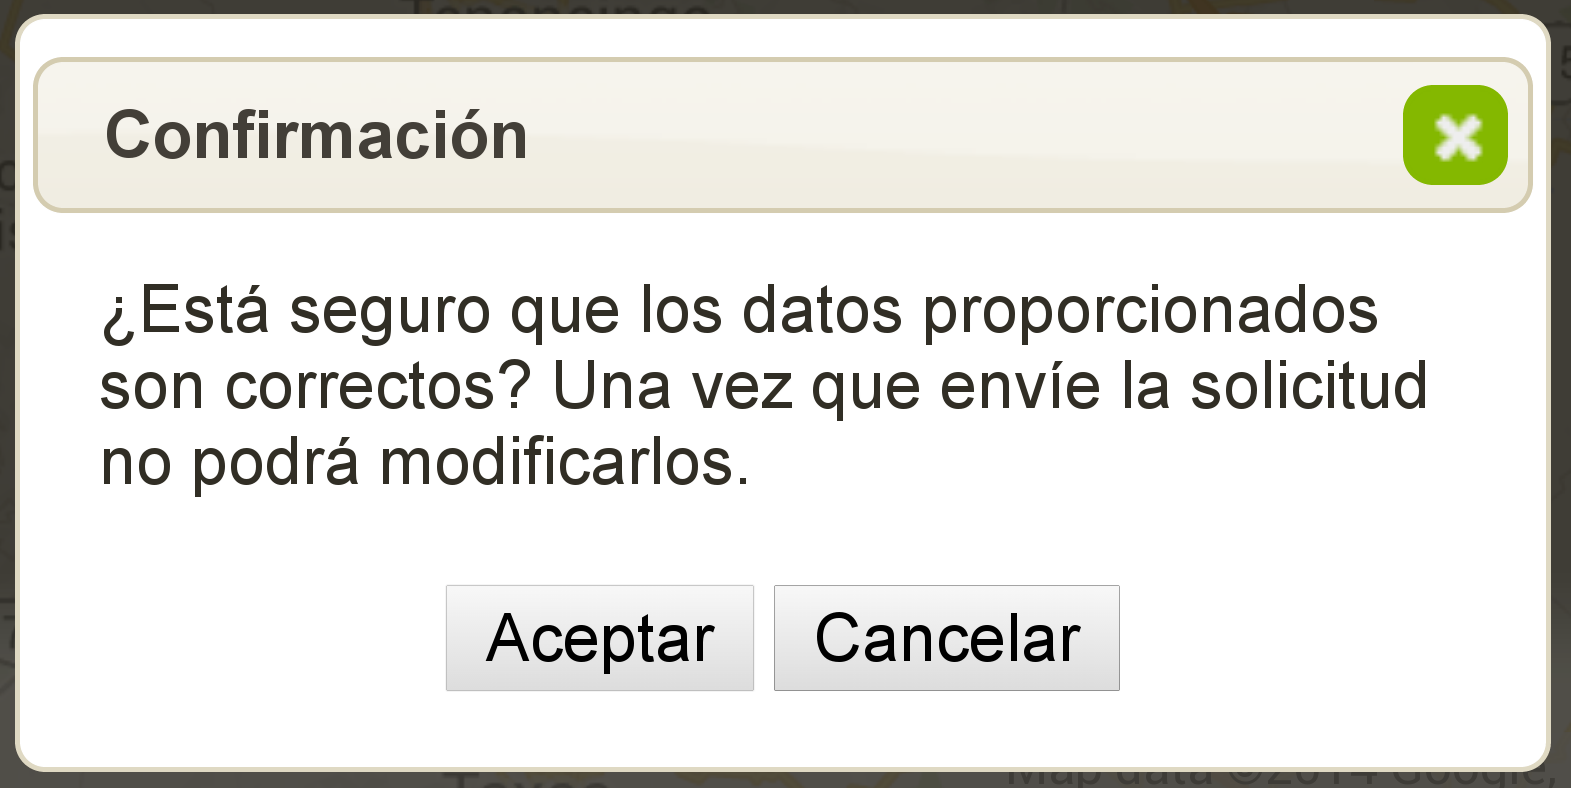
\includegraphics[width=.7\textwidth]{images/pantallas/general/pantallaEmergente}}
	  \caption{Pantalla emergente.}
	  \label{fig:pantallaEmergente}
	  \cdtLabel{fig:pantallaEmergente}{}
	\end{center}
      \end{figure}
  

      %----------------------------------------------------------
      \subsubsection{Captcha}
      \label{ch:Interaccion:Captcha}

      En la figura \ref{fig:captcha} se muestra el segmento de pantalla ``Captcha'', en la cual se mostrará una cadena de texto de 6 caracteres  para validar que la interacción con el sistema no esté dada por un robot.
      \begin{figure}[htbp!]
	  \begin{center}
	      \fbox{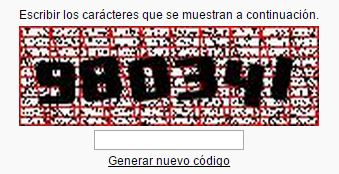
\includegraphics[width=.7\textwidth]{images/pantallas/general/CAPTCHA}}
	      \caption{Captcha}
	      \label{fig:captcha}
	      \cdtLabel{fig:captcha}{}
	  \end{center}
      \end{figure}

%    \subsubsection{Tabla de selección de múltiple}
%      Este componente permite realizar una selección múltiple de valores, los cuales corresponden a las opciones disponibles en un catálogo. Es posible realizar búsquedas y seleccionar la cantidad de registros a mostrar por página, así como navegar el paginado con las opciones ``Anterior'' y ``Siguiente''.
%      Muestra los botones \cdtButton{Aceptar} y \cdtButton{Cancelar}, que permiten confirmar la selección o cancelarla respectivamente.
%      En la figura \ref{fig:tablaSeleccion} se muestra un ejemplo de este componente. 
%       \begin{figure}[htbp!]
% 	  \begin{center}
% 	      \fbox{\includegraphics[width=.7\textwidth]{images/pantallas/general/tablaSeleccion}}
% 	      \caption{Tabla de selección múltiple.}
% 	      \label{fig:tablaSeleccion}
% 	      \cdtLabel{fig:tablaSeleccion}{}
% 	  \end{center}
%       \end{figure}
  
  
\subsection{Organización}
Las funcionalidades del sistema se encuentra organizadas por menús. Cada actor accede a un menú diferente dependiendo de su perfil, ya que este describe el ciclo de trabajo y las funciones que el actor puede realizar.
%En la parte superior de la pantalla en la interfaz de usuario, se mostrará un menú correspondiente a cada perfil que ingrese al sistema, el cual tendrá las opciones ``Inicio'', ``Información general'', ``Diagnóstico'', ``Plan de acción'' y ``Seguimiento y acreditación'', además de las opciones a las que cada perfil tiene acceso. La opción ``Inicio'' dirige a la pantalla de bienvenida de sistema, mostrada en la figura~\ref{fig:inicio}. La opción ``Información general'' dirige a la pantalla de administración de información escolar  mostrada en la figura~\ref{IUR 5}.  La opción ``Diagnóstico'' dirige a la pantalla de administración de información escolar  mostrada en la figura~\ref{IUD 1}.  La opción ``Plan de acción'' dirige a la pantalla de administración de información escolar  mostrada en la figura~\ref{IUP 1}.  La opción ``Seguimiento y acreditación'' dirige a la pantalla de administración de información escolar  mostrada en la figura~\ref{IUS 5}. A continuación se describen los menús correspondientes a 
cada perfil en el sistema.

\subsubsection{Menú del Coordinador del programa}

    En la figura~\ref{MN2} se muestran las opciones del menú superior que serán visibles para el actor \cdtRef{actor:usuarioEscuela}{Coordinador del programa}. Las opciones del menú se enlistan a continuación:

    \begin{Citemize}
      \item Inicio
      \item Información general
      \item Información base para indicadores
      \item Plan de acción
      \item Seguimiento y acreditación
      \item Indicadores
    \end{Citemize}
    
    \IUfig[.9]{menus/coordinador}{MN2}{Menú del Coordinador del programa}

   
 Al seleccionar la opción ``Información general'' se desplegarán las opciones que se muestran en la figura~\ref{MN2.1} y se enlistan a contiuación: 
    \begin{Citemize}
		\item Información escolar
		\item Responsable del programa		
		\item Integrantes de línea de acción
		\item Coordinador del programa				
    \end{Citemize}

    \IUfig[.9]{menus/coordinador_general}{MN2.1}{Menú del Coordinador del programa. Submenú de ``Información general''.}

 Al seleccionar la opción ``Información base para indicadores'' se desplegarán las opciones que se muestran en la figura~\ref{MN2.2} y se enlistan a contiuación: 
    \begin{Citemize}
		\item Agua
		\item Residuos sólidos
		\item Energía
		\item Biodiversidad
		\item Ambiente escolar		
		\item Consumo responsable		
		\item Enviar información base
    \end{Citemize}


    \IUfig[.9]{menus/coordinador_diagnostico}{MN2.2}{Menú del Coordinador del programa. Submenú de ``Información para indicadores''.}

 Al seleccionar la opción ``Plan de acción'' se desplegarán las opciones que se muestran en la figura~\ref{MN2.3} y se enlistan a contiuación: 
    \begin{Citemize}
		\item Objetivos
		\item Enviar plan de acción
    \end{Citemize}

    \IUfig[.9]{menus/coordinador_plan}{MN2.3}{Menú del Coordinador del programa. Submenú de ``Plan de acción''.}

 Al seleccionar la opción ``Seguimiento y acreditación'' se desplegarán las opciones que se muestran en la figura~\ref{MN2.4} y se enlistan a contiuación: 
    \begin{Citemize}
		\item Seguimiento del plan de acción
		\item Enviar informe de seguimiento
		\item Acreditación en el programa
    \end{Citemize}
    \IUfig[.9]{menus/coordinador_seguimiento}{MN2.4}{Menú del Coordinador del programa. Submenú de ``Seguimiento y acreditación''.}